\section{Introduction}
\subsection{Context \& Motivation}
%Introduce most of the concepts around money in electric transportation/urbanization/environmental aspects from the presentation, e.g. "why is this needed"
\subsubsection{The RipStik}
\subsection{Problem Definition}
\subsection{Technical Background}
\subsubsection{Euler Angles}
\subsubsection{Lagrangian Mechanics}
\subsubsection{Euler-Lagrange Equations}
\subsubsection{Nonholonomic Constraints}
\subsubsection{Numeric Integration}
\subsubsection{Linear Quadratic Regulator Control}
The linear quadratic regulator (LQR) algorithm is a method in control theory used to technique used to determine the optimal control gains for a state feedback controller for a linear system with a quadratic cost function. \textbf{CITE LAB MANUAL OR SOMETHING}

For the purpose of this project, linear control systems $\Sigma$ of the form
\begin{equation}
\dot{x}(t) = Ax(t) + Bu(t)
\end{equation}
where $A \in \R^{m \times m}$ and $B \in \R^{m \times l}$ are considered.
The associated quadratic cost function is then 
\begin{equation}
\eta(u) = \int_{0}^{\infty}x^{T}(t)Qx(t)+u^{T}(t)u(t)dt
\end{equation}
where $Q \in \R^{m \times m}$ is the weighting matrix associated with the degrees of freedom and their derivatives $(q, \dot{q})$ in the system. Note that no weightings are associated with the control inputs at this stage, though they may be necessary when considering the broader design impacts (see section \textbf{FILL IN SECTION REF}). Tuning the cost function weighting matrix $Q$ allows emphasis to be placed on stabilization of certain degrees of freedom to better meet design goals for the particular application.

The optimal control gains $K$ are then computed from
\begin{equation}
K = B^{T}X_{r}
\end{equation}
where  $X_{r}$ is the solution to the continuous Riccati equation \textbf{CITE MATHEMATICA DOCS FOR RICCATISOLVE}
\begin{equation}
A^{T}X_{r} + X_{r}A - (X_{r}B)(B^{T}X_{r}) + Q = 0.
\end{equation}

\subsection{Literature Review}
\subsubsection{A Nonlinear Mathematical Model for a Bicycle}
To gain a clearer perspective of the overall procedure and concepts involved in modeling a complex mechanical system of this nature, a number of similar mathematical models for other modes of personal transportation were analyzed.
In particular, \textit{A Nonlinear Mathematical Model for a Bicycle} \cite{bicycle} provides a clear example of establishing the necessary coordinate systems and transformation matrices associated with the interconnections and internal angles within the bicycle.
This model includes the rolling dynamics of the wheels and discusses the minutiae of elements like the wheel crown radius, demonstrating the complexity they add to the model before removing these elements to provide a more manageable model.
The final model is also constructed under the assumption that the rider remains stable and upright, allowing the roll angle of the bicycle to be linearized, further facilitating interpretation of the final modeling results. 
%%%%%%%%%%%%%%%%%%%%%%%%%%%%%%%%
%%%%SHOULD WE INCLUDE AN IMAGE
%%%%Is wheel crown radius not self explanatory
%%%%%%%%%%%%%%%%%%%%%%%%%%%%%%%%

\subsubsection{Modeling and Control of Casterboard Robot}
In the paper \textit{Modeling and Control of Casterboard Robot} \cite{robot}, Kinugasa et al. discuss similar concepts and their application in the context of a casterboard, however, the overarching goals and product were distinct from the defined problem.
The group from Osaka University developed a highly simplified model, omitting the problem of stability and simplifying the dynamics of the caster rotation using a holonomic constraint. 
They then used this to develop a locomotion control method for the casterboard before implementing, testing and tuning it on a physical robot constructed to match the geometry of the casterboard.

%%%%%%%%%%%%%%%%%%%%%%%%%%%%%%%%
%%%%SHOULD WE INCLUDE AN IMAGE
%%%%%%%%%%%%%%%%%%%%%%%%%%%%%%%%
\subsubsection{Nonholonomic Constraints \& Linearization}
%%%%%%%%%%%%%%%%%%%%%%%%%%
%%%%
%%%%FUCK IT I'LL DO THIS LATER IDK
%%%%
%%%%%%%%%%%%%%%%%%%%%%%%%%
\subsection{Software Tools}
\subsubsection{Mathematica}
Due to the complex nature of the model and the large number of degrees of freedom needed to accurately model the behavior of the RipStik, a powerful symbolic computation tool is required to derive and manipulate the expressions. 
Mathematica was ultimately selected over other options such as Maple and the Matlab Symbolic toolbox due to the combination of robust symbolic and numeric computation features with easy to use visualization features for graphically displaying the various systems developed over the course of the project.
It also provided equivalent or better performance with thorough documentation and examples compared to competitors.
%%%%%%%%%%%%%%%%%%%%%%%%
%%%%DO I NEED A SOURCE FOR BETTER PERFORMANCE
%%%%%%%%%%%%%%%%%%%%%%%%
\subsubsection{Three.JS}
While all of the more simple visualizations were constructed directly in Mathematica, an external tool was constructed to animate the full RipStik system in a more attractive and visually intuitive manner. 
The application is javascript based and operated via the web browser, allowing the user to upload a .csv (comma separated value) file of numeric output from the RipStik simulation and returning an animation of the results on a 3 dimensional RipStik model. 
This allows easy validation of the results by inspection, particularly for complex motions where graphs of the angles and positions may not make the full system behavior immediately obvious.
The process used to generate these animations in the application is shown in Figure \ref{fig:ThreeJsFlow}.

%%Define the two block types and arrow type for our flow diagram
\tikzstyle{startstop} = [rectangle, rounded corners, minimum width=3cm, minimum height=1cm,text centered, draw=black, fill=white]
\tikzstyle{process} = [rectangle, minimum width=3cm, minimum height=1cm, text centered, draw=black, fill=white]
\tikzstyle{arrow} = [thick,->,>=stealth]
\begin{center}
	\begin{figure}[!htb]
		\begin{center}
			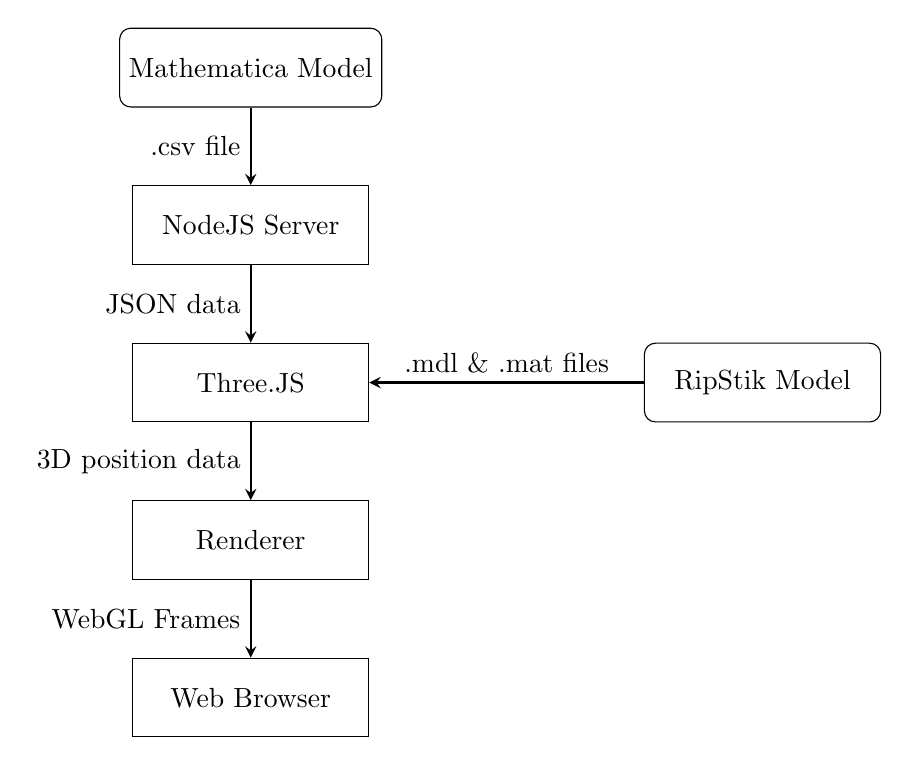
\begin{tikzpicture}[node distance=2cm]
				\node (WA) [startstop] {Mathematica Model};
				\node (Srvr) [process, below of=WA] {NodeJS Server};
				\node (Three) [process, below of=Srvr] {Three.JS};
				\node (Mdl) [startstop, right of=Three, xshift=4.5cm] {RipStik Model};
				\node (Rndr) [process, below of=Three] {Renderer};
				\node (Brwsr) [process, below of=Rndr] {Web Browser};

				\draw [arrow] (WA) -- node[anchor=east] {.csv file} (Srvr);
				\draw [arrow] (Srvr) -- node[anchor=east] {JSON data} (Three);
				\draw [arrow] (Mdl) -- node[anchor=south] {.mdl \& .mat files} (Three);
				\draw [arrow] (Three) -- node[anchor=east] {3D position data} (Rndr);
				\draw [arrow] (Rndr) -- node[anchor=east] {WebGL Frames} (Brwsr);
			\end{tikzpicture}
		\end{center}
	\caption{RipStik animation tool data flow summary}\label{fig:ThreeJsFlow}
	\end{figure}
\end{center}
The core of the application is ThreeJS, a javascript WebGL library that allows the 3D model to be loaded from a .mdl file (the set of 3D dimensional points that forms the shape) and .mat file (the colors/materials to be overlaid on the shape) then animated using rotations and translations in a standard Cartesian coordinate system.